\chapter{Introduction to the problem}
\label{ch:introduction_to_the_problem_spark}%
In this part, we implement a bibliographic database relying on the infrastructure provided by Apache Spark.
Apache Spark is a scalable platform for performing complex analytics.
It manages data within a distributed system and this guarantees fast processing, fault tolerance, and high scalability.
The framework allows using different technologies for implementing the database.
We use a logic paradigm that looks like the relational one.
We rely on the \verb|Dataframe| object, which can be imagined as a table containing data but with a lot of enhancing features.
We use \verb|pyspark|, which is the Python library for creating and managing the database in Spark, in order to translate the conceptual model defined in chapter 2.
Articles, authors, and various types of publications become the tables containing the instances of the data.
Apache Spark is a good approach when dealing with huge amounts of data and in the real world, a bibliography database contains a lot of papers.
On the other hand, in our application, we use a small subset of the published papers and we are running Spark only on one machine so we are not fully exploiting the real power of the platform.
In treating this problem from a new point of view, though, we try to take advantage of the functions available in \verb|pyspark| and of its features as much as we can.


\chapter{Dataset structure}
\label{ch:dataset_structure_spark}%
In this part, we implemented a database with a very similar structure to the ER model described in chapter 2.
We decided to create six different tables:
\begin{itemize}
    \item \textbf{df\_papers} is the table containing all the attributes concerning a single paper.
    With respect to the ER model here we have \verb|publication_type| and \verb|publication_id| that are necessary in order to do the join with a certain type of publication; \verb|page_start|; \verb|page_end|; \verb|date| instead of \verb|year|; and \verb|references| which is a list that substitutes the corresponding relationship;
    we also have the lists of \verb|fos| and \verb|keywords| related to the paper and the other attributes identified in the modeling part of the bibliography;
    \item \textbf{df\_aut} is the table related to authors and contains \verb|email| and \verb|bio| in addition to the ER model;
    \item \textbf{df\_aff} is the table with the author's affiliation when the paper was written, this table maps the
    \verb|writes| relationship;
    \item \textbf{df\_journals} is the table with the journals;
    \item \textbf{df\_books} is the table with the books;
    \item \textbf{df\_conferences} is the table with the conferences.

    We decided to represent the entity Publication with the sub-entities, for this reason, all contain \verb|publication_id|  and \verb|publication_type| that are used in the join with \verb|df_papers|.
    The attribute \verb|name| in Publication in the ER model, as well as in other parts of the document, is called \verb|venue|.
\end{itemize}
The following table shows all the fields associated with their respective type, meaning, and table.
\begin{table}[H]
    \begin{center}
        \begin{tabular}{| c | c | c | p{0.25\linewidth} |}
            \hline
            \textbf{Field name} & \textbf{Type}   & \textbf{Description}  & \textbf{Table} \T\B                                      \\
            \hline \hline
            publication\_id     & long            & publication id        & df\_papers, df\_books, df\_journals, df\_conferences\T\B \\
            paper\_id           & string          & paper ID              & df\_papers, df\_aff\T\B                                  \\
            title               & string          & paper title           & df\_papers\T\B                                           \\
            keywords            & array of string & paper keywords        & df\_papers\T\B                                           \\
            fos                 & array of string & paper fields of study & df\_papers\T\B                                           \\
            references          & array of string & paper references      & df\_papers\T\B                                           \\
            page\_start         & integer         & start page            & df\_papers\T\B                                           \\
            page\_end           & integer         & end page              & df\_papers\T\B                                           \\
            lang                & string          & paper language        & df\_papers\T\B                                           \\
            doi                 & string          & paper DOI             & df\_papers\T\B                                           \\
            url                 & array of string & paper URLs            & df\_papers\T\B                                           \\
            abstract            & string          & paper abstract        & df\_papers\T\B                                           \\
            publication\_type   & string          & paper type            & df\_papers\T\B                                           \\
            date                & timestamp       & publication date      & df\_papers\T\B                                           \\
            author\_id          & string          & author ID             & df\_aut, df\_aff\T\B                                     \\
            name                & string          & author name           & df\_aut\T\B                                              \\
            email               & string          & author email          & df\_aut\T\B                                              \\
            bio                 & string          & author short bio      & df\_aut\T\B                                              \\
            organization        & string          & author affiliation    & df\_aff\T\B                                              \\
            venue               & string          & publication name      & df\_books, df\_journals, df\_conferences\T\B             \\
            isbn                & string          & book ISBN             & df\_books\T\B                                            \\
            publisher           & string          & publisher name        & df\_books, df\_journals\T\B                              \\
            volume              & integer         & journal volume        & df\_journals\T\B                                         \\
            issue               & integer         & journal issue         & df\_journals\T\B                                         \\
            issn                & string          & journal ISSN          & df\_journals\T\B                                         \\
            location            & string          & conference location   & df\_conferences\T\B                                      \\
            \hline
        \end{tabular}
        \\[8pt]
        \caption{Description of the fields with related type, meaning, and table.}
        \label{tab:dataset_structure}%
    \end{center}
\end{table}
Below we provide the actual schema of each table obtained by invoking the function \verb|printSchema()|.
\begin{figure}[H]
    \begin{center}
        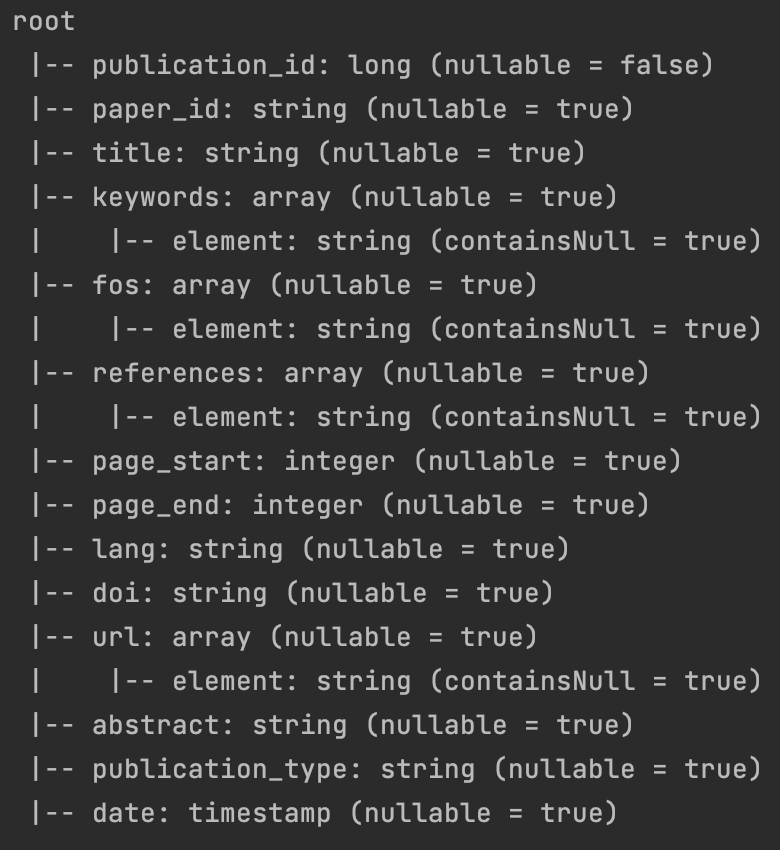
\includegraphics[width=0.6\linewidth]{ImagesSpark/paper_schema}
        \caption{Paper table - df\_papers.}
        \label{fig:figure4_1}%
    \end{center}
\end{figure}
\begin{figure}[H]
    \begin{center}
        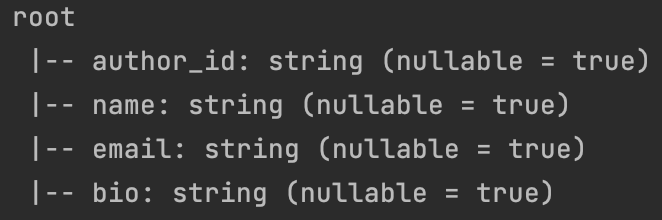
\includegraphics[width=0.6\linewidth]{ImagesSpark/author_schema}
        \caption{Author table - df\_aut.}
        \label{fig:figure4_2}%
    \end{center}
\end{figure}
\begin{figure}[H]
    \begin{center}
        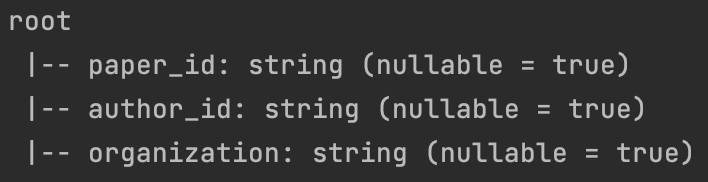
\includegraphics[width=0.6\linewidth]{ImagesSpark/affiliation_schema}
        \caption{Affiliation table - df\_aff.}
        \label{fig:figure4_3}%
    \end{center}
\end{figure}
\begin{figure}[H]
    \begin{center}
        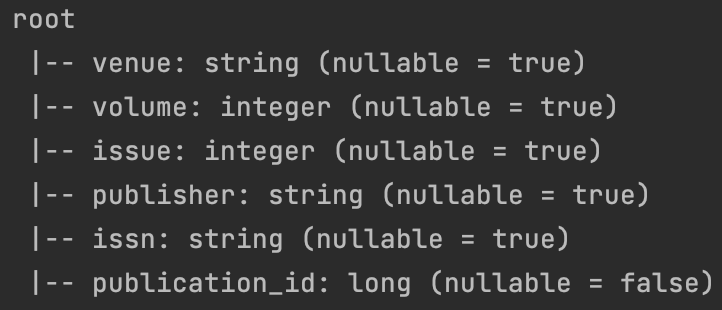
\includegraphics[width=0.6\linewidth]{ImagesSpark/journal_schema}
        \caption{Journal table - df\_journals.}
        \label{fig:figure4_4}%
    \end{center}
\end{figure}
\begin{figure}[H]
    \begin{center}
        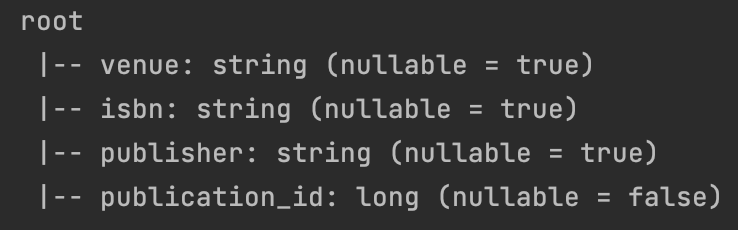
\includegraphics[width=0.6\linewidth]{ImagesSpark/book_schema}
        \caption{Book table - df\_books.}
        \label{fig:figure4_5}%
    \end{center}
\end{figure}
\begin{figure}[H]
    \begin{center}
        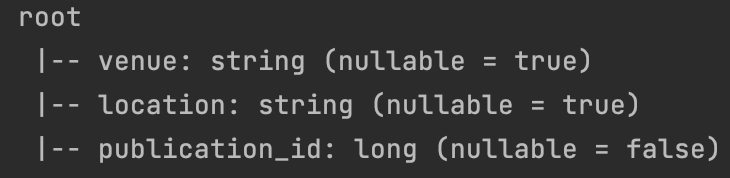
\includegraphics[width=0.6\linewidth]{ImagesSpark/conference_schema}
        \caption{Conference table - df\_conferences.}
        \label{fig:figure4_6}%
    \end{center}
\end{figure}


\chapter{Data upload}
\label{ch:data_upload_spark}%
The library \verb|pyspark| provides many functions to upload data stored in different formats.
In our case, the dataset was stored in the JSON format, specifically, it is the one used in MongoDB except for some minor changes, so we used the API for this format.
To upload the data we used the object \verb|DataFrameReader|, which is accessible as an attribute of our \verb|SparkSession| instance.
More specifically using the \verb|options| method we specified some instructions on how to read the data, and with the \verb|schema| method we supplied a specific schema for the data to be read in order to keep only the fields specified in it.
We created a DataFrame for each entity of our ER diagram of chapter 2 and we also translated the many-to-may relationship \verb|Writes| into a table to keep track of the \verb|affiliation| field.
For each table, we did some additional filtering on its attributes in order to clean the data and we also did some minor changes that we will now explain.
The dataset we inherited from the MongoDB part had a simple structure: a single document, the paper, where all other entities (authors, publication, affiliation) were stored as sub-documents, a collection of sub-documents or simple fields that are present only when needed.
Therefore, we have to extrapolate the information regarding the authors and the publications from the papers.
In particular, a more complex process was applied to build the dataframes containing information concerning books, conferences, and journals.
The following sections briefly explain the processing done within the upload step for each entity contained in the spark database and the reasoning behind it.


\section{Author table}
\label{sec:author_table_spark}%
This table was created by extracting from each Paper document the array containing the authors' documents, with their fields.
To do this, we first had to load the data using the load process described in the section before.
Secondly, we unwrapped each array using the \verb|explode| function to have a table where each row represents the author document.
Finally, we did some filtering on null values and some minor operations, such as renaming, deleting duplicates, or dropping columns.


\section{Paper, Book, Conference, Journal tables}
\label{sec:paper_book_conference_journal_tables}%
To load the data relevant to the entities Book, Conference, and Journal we had to address two issues: how to extract and integrate the different types of publications and how to link each paper to the publication medium in which it was published.
The first issue is solved by uploading in the DataFrame of each publication type only the fields regarding that specific entity, namely the attributes present in the ER model of section 2, and filtering each DataFrame removing the duplicate rows.
We also imposed that the fields have to be not null.
To overcome the second issue we opted to introduce a ``foreign key'' column in the paper DataFrame which stores the unique identifier of the publication medium where it was published.
To make the linking with the ``foreign key'' approach work, we added a unique identifier to each single publication instance cleaned through the previous step.
This identifier is generated using a hashing function, specifically the function \verb|xxhash64| present in the pyspark library, which uses the 64-bit variant of the xxHash algorithm.
We fed this function with the columns we identified as the primary key, to generate the unique identifier.

The other possible solution we thought of was the creation of an array inside each publication containing all the papers present inside it.
In the end, we adopted the first solution because our focus is on the paper, which is the main entity of the database and we assume that the vast majority of the queries will probably have the paper as a starting point, and then retrieve all the information correlated to the paper.
In this way, opting for the first solution and considering the assumption mentioned here, the queries done on the papers should be more efficient.

The process we used to upload Books, Journals and Conferences is the following:
\begin{enumerate}
    \item Upload the paper documents from the JSON input file in a DataFrame with the structure we defined in chapter 12, except for the attribute \verb|publication_id| that will be added later;
    \item For each type of publication:
    \begin{enumerate}
        \item Upload the data from the JSON file keeping only the fields relative to a single publication type and the field \verb|_id|, which is the identifier of a paper;
        \item Filter out the rows of the dataframe which have the publication's identifying fields set to null, namely \verb|('venue', 'volume', 'issue', 'issn')| for the journals, \verb|('isbn', 'venue')| for the books and \verb|('venue')| for the conferences;
        \item Group each publication by the uniquely identifying fields and collect the the other fields, especially \verb|_id|, in lists;
        \item Select the first element of the list of non-identifying attributes, \verb|'publisher'| for journals and books, and \verb|'location'| for the conferences.
        This choice is motivated by the fact that these fields were set using random strings extracted from some datasets we found on the web.
        In real scenarios, where we assume to have meaningful data, the best thing to do would be to implement a strategy that keeps the last inserted value for the field or the one that appears the most;
        \item Create the publication identifier (field \verb|publication_id|) using the previous explained hash function;
        \item Create a new DataFrame containing papers, constructed by joining the previous imported Paper DataFrame (Point 1) with the DataFrame of the publication on the field \verb|_id|, which is the paper identifier.
        In this way we attach to the newly generated Paper DataFrame the \verb|publication_id| field, linking the paper to it's publication.
        Notice that in order to perform the join we first have to \textit{explode} the field \verb|_id| of the publication DataFrame;
    \end{enumerate}
    \item At this step of the process, in addition to the dataframes for the journals, for the books and for the conferences we also have other the three newly created paper dataframes obtained by the joining operations.
    These lastly mentioned dataframes have the same structure of the originial one with the addition of the fields that identify the paper publication.
    By merging this the three dataframes we obtain the final dataframe of the papers.
\end{enumerate}
In addition to this major operation some minor ones were performed, such as renaming or dropping columns, but these are straightforward to understand, so we won't discuss them any further in this report.


\section{Affiliation table}
\label{sec:affiliation_table}%
This table was created by uploading, from the JSON file, only the identifiers of the papers and their array of authors keeping the id of the author and the organization to which they were affiliated.
After filtering the null values, the authors' array is expanded, using the \verb|explode()| function.
As before, some other minor operations were also done, such as renaming or dropping of columns.


\chapter{Commands and queries}
\label{ch:commands_and_queries_spark}%


\section{Commands}
\label{sec:commands_spark}%

\begin{enumerate}
    \item \textbf{Add a new paper to the DataFrame} \\
    With this command, we want to show how to add a new row to our Paper DataFrame.
    In our example, we suppose that the paper has been saved in a JSON file and has a structure consistent with the schema defined in chapter 12 for the input dataset.
    This way, we can reuse the loading procedure used before for the entire dataset loading.
    We first create a new DataFrame for the single paper.
    Once the paper is loaded, we can proceed to extract other information relevant to the paper, like the authors, and the publication medium but we don't show this part here to have a more concise description (the actual implementation is present on the notebook).
    After this operation, we proceed to insert the foreign\_key associated with the publication medium in the DataFrame containing our paper to insert.
    This operation is done using the \verb|select| method so we can insert the column as the first one to stay uniform with the structure because in spark even the order of the columns is important.
    To create the column from a literal value we use the function \verb|lit|.
    Now the new paper is ready to be added, we have only to first check if the paper is already present in the DataFrame, and we do this by filtering by \verb|paper_id| and verifying that the collection is empty.
    Then to add the paper we use the method \verb|union| which is applied to DataFrame and returns a new DataFrame containing the union of rows of both DataFrames.
    \begin{lstlisting}[label={lst:command1spark}]
new_paper_file = 'single_paper.json'

new_paper = spark.read.options(**OPTIONS)
.json(new_paper_file, schemaPaper)\
.withColumnRenamed("_id", "paper_id")

# Other code for loading publication, authors, etc
# ...

# Inserting foreign_key at position 0
new_paper = new_paper.select(lit(foreign_key).alias('publication_id'), '*')

paper_id = new_paper.head(1)[0].asDict()['paper_id']

if df_papers.filter(col('paper_id') == paper_id).collect() == []:
df_papers = df_papers.union(new_paper)
    \end{lstlisting}
    \item \textbf{Update one single row of a dataframe or multiple rows} \\
    The word update has to be intended as the creation of a new dataframe instance which is generated from the previous data changed in the way we want.
    Indeed, the Dataframe data structure, available in Spark, is immutable so it cannot be modified.
    Since the modifications are not allowed, to update a single entry the process is a little longer than the one used on other databases.

    The update process can be useful for uploading papers when new data enter the database or when parts of the data were wrong and need to be corrected.
    There may be many handmade ways to update a dataframe since there are no standard methods.
    All of them are similar in their underlying idea.

    The command modifies the DOI and URL of a paper with an identifier equal to \verb|'53e997e4b7602d9701fdb48a'|.
    For doing this operation we first filter the dataframe keeping only the row to be modified.
    We add a column for each value we want to insert under the name \verb|new_fieldName|.
    Then we drop the old columns containing the previous values and we rename the new columns with the name of the old ones.
    Finally, we make the union between the entire dataframe, without the row we want to modify, and the new entry.
    The \verb|union| function allows to merge two DataFrame with the same schema;
    if the two structures are different, then the function gives an error.

    The function \verb|lit| is used for creating a new column containing a literal, namely a constant value.
    The function \verb|array| is used for creating a new array column.
    \begin{lstlisting}[label={lst:command2spark}]
from pyspark.sql.functions import lit, array

updated_df_papers = df_papers\
.filter(col('paper_id') == '53e997e4b7602d9701fdb48a')
updated_df_papers = updated_df_papers\
.withColumn('new_doi', lit('10.1007/11944577_37'))\
.withColumn('new_url', array([lit('https://link.springer.com/chapter/10.1007/11944577_37')]))
updated_df_papers = updated_df_papers\
.drop(col('doi')).drop(col('url'))\
.withColumnRenamed('new_doi', 'doi')\
.withColumnRenamed('new_url', 'url')

updated_df_papers = df_papers.filter(col('paper_id') != '53e997e4b7602d9701fdb48a').union(updated_df_papers)
updated_df_papers.filter(col('paper_id') == '53e997e4b7602d9701fdb48a').select('paper_id', 'title', 'doi', 'url').show(truncate = False)
    \end{lstlisting}
    An analogous method can be applied when we want to update multiple rows following some rule.
    In this case, the filter will keep many rows and not just one.
    \begin{figure}[H]
        \begin{center}
            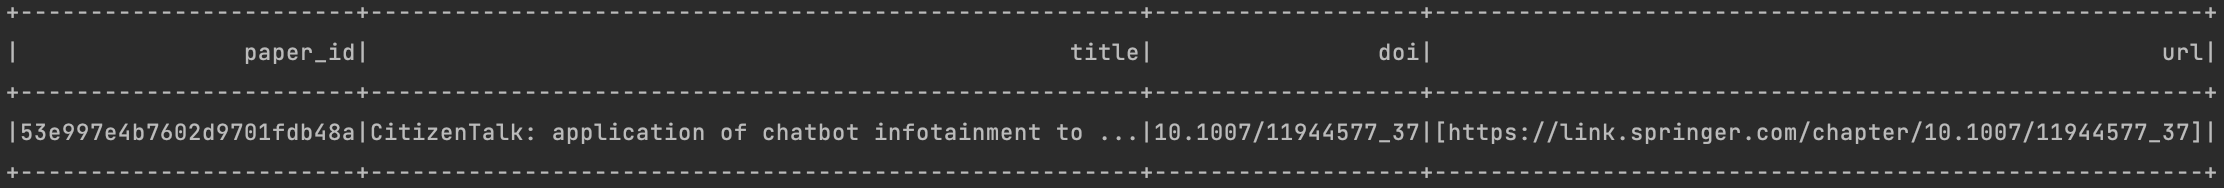
\includegraphics[width=0.9\linewidth]{ImagesSpark/command2spark}
            \label{fig:command2spark}%
        \end{center}
    \end{figure}
    \item \textbf{Remove an entire column} \\
    In Spark, we can remove an entire column from a data frame due to deleting information that is no more informative.
    In these cases, we delete them to free memory for new data.

    To realize our objective, we use the function \verb|drop|, which removes entirely values associated with a field of the data frame.

    In our database, we can use the explained function over the column \verb|lang| because we have realized that all the papers have the same value, \verb|en|.
    Then, we print the schema of the data frame to see if the function ran properly.
%and finally, we visualize an example of the new paper by calling the \verb|show| operation.
    \begin{lstlisting}[label={lst:command3spark}]
df_papers_without_lang = df_papers \
.drop('lang')

df_papers_without_lang.printSchema()
df_papers_without_lang.show(1)
    \end{lstlisting}
    \begin{figure}[H]
        \begin{center}
            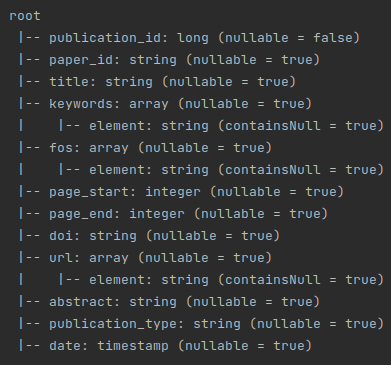
\includegraphics[width=0.6\linewidth]{ImagesSpark/command3spark}
            \label{fig:command3spark}%
        \end{center}
    \end{figure}
    \item \textbf{Delete all the papers published before a certain year} \\
    In order to delete from the DataFrame \verb|df_papers| the rows that represent papers published before a certain year is necessary to create a new DataFrame extracting from the original one only the papers that satisfy the desired condition.
    We decided to remove all the papers that were published before the \verb|1950| because we consider them obsolete.
    To check the year in which a paper was published is necessary to use the function \verb|year| in order to extract the information from the \verb|date|, that is of type \verb|TimeStamp|.
    Based on the condition \verb|year('date') > '1950'| we drop with the \verb|where| clause all the rows that do not satisfy it, saving all the others in the new DataFrame.
    Finally, with the following command, we show the result of these actions and we present the new \verb|df_papers| ordering the visualization by date, so it is immediately visible that there are no papers realized before \verb|1951|.
    \begin{lstlisting}[label={lst:command4spark}]
from pyspark.sql.functions import year

df_papers = df_papers\
.filter(year('date') > '1950')

df_papers.select('title', 'publication_type', 'date')\
.orderBy('date')\
.show(truncate = False)
    \end{lstlisting}
    \begin{figure}[H]
        \begin{center}
            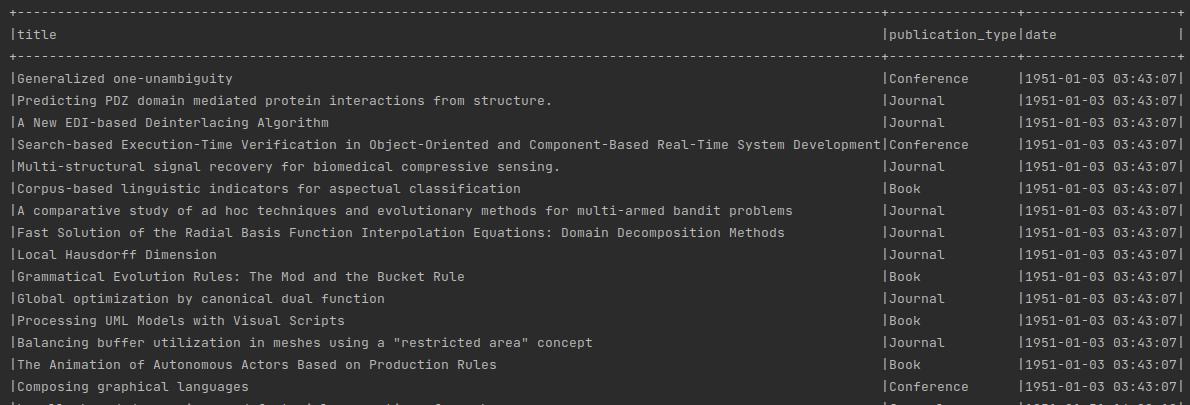
\includegraphics[width=0.9\linewidth]{ImagesSpark/command4spark}
            \label{fig:command4spark}%
        \end{center}
    \end{figure}
    \item \textbf{Create a new column with the paper's total number of pages} \\
    With this command, we create a new DataFrame \verb|df_papers_total_pages| starting from \verb|df_papers| but with an additional column called \verb|total_pages| using the function \verb|withColumn()|.
    This new column contains the total number of pages of the paper computed as the difference between \verb|pages_end| and \verb|page_start| by doing also some consistency checks on these values.
    Then only some fields are displayed just for better reading.
    \begin{lstlisting}[label={lst:command5spark}]
df_papers_total_pages = df_papers \
.filter((col('page_start') >= 0) & (col('page_end') >= 0) & (col('page_start') <= col('page_end'))) \
.withColumn('total_pages', col('page_end') - col('page_start'))

df_papers_total_pages \
.select(col('title'), col('page_start'), col('page_end'), col('total_pages')) \
.show(5, truncate=False)
    \end{lstlisting}
    \begin{figure}[H]
        \begin{center}
            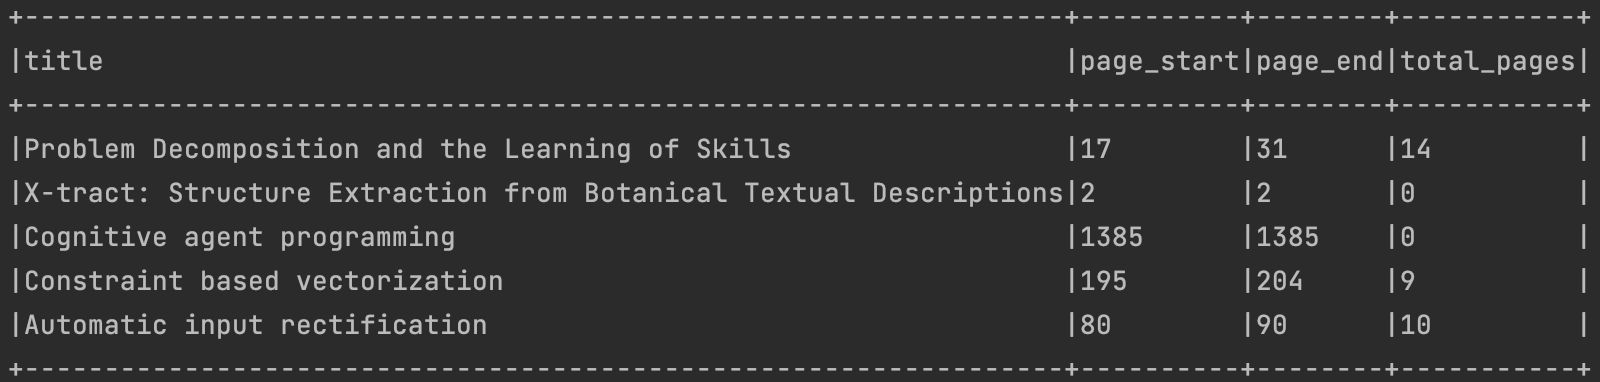
\includegraphics[width=0.9\linewidth]{ImagesSpark/command5spark}
            \label{fig:command5spark}%
        \end{center}
    \end{figure}
\end{enumerate}


\section{Queries}
\label{sec:queries_spark}%
\begin{enumerate}
    \item \textbf{Retrieve all papers published on a specific issue and volume of a Journal} \\
    With this simple query, we want to retrieve all the papers published on a specific issue and on a specific volume of a specific Journal.
    The specifics of the journal are saved in variables to be used later.
    To perform the query we first do a filtering (which is equivalent to a \verb|WHERE|) on the DataFrame containing the journals, to extract only the row concerned with our paper.
    After that, we perform the default \verb|inner| join with the papers' DataFrame.
    Notice that, besides specifying the column on which to perform the join, we do an additional check on the \verb|publication_type| to ensure that the join operations are done only for journals.
    This type of checking is made easy thanks to the possibility offered by Spark to specify more complex join conditions.
    \begin{lstlisting}[label={lst:query1spark}]
venue, volume, issue = ('BMC Bioinformatics', '14', '1')

df_papers_q1 = df_journals\
.filter((col('venue') == venue) &
(col('volume') == volume) &
(col('issue') == issue))\
.join(df_papers,
(df_journals['publication_id'] == df_papers['publication_id']) &
(df_papers['publication_type'] == 'Journal')
)

df_papers_q1.select(['paper_id', 'title']).show(truncate=60)
    \end{lstlisting}
    \begin{figure}[H]
        \begin{center}
            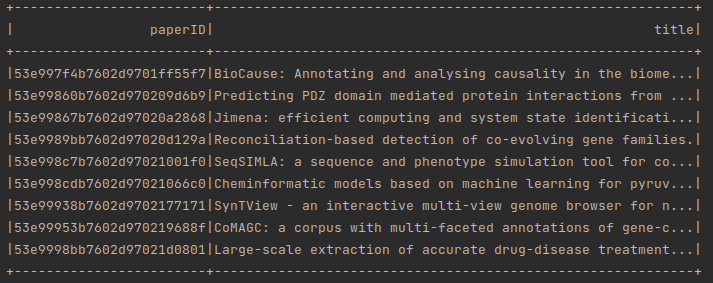
\includegraphics[width=0.9\linewidth]{ImagesSpark/query1spark}
            \label{fig:query1spark}%
        \end{center}
    \end{figure}
    \item \textbf{Papers written in the last 20 years and containing a chosen string within a keyword} \\
    Find the papers written in the last twenty years whose keywords contains at least one keyword having \verb|artificial| as substring.
    We require that these papers have the DOI set to a not null value.
    The results are ordered ascending by the date and only 15 elements are printed.

    For filtering a Dataframe variable we can use the function \verb|filter(condition)| of \verb|pyspark| library.
    This function returns a new DataFrame containing only the rows which make the condition true and eliminate the others.
    We can use the function \verb|like(string)| as a filtering condition on a column of the DataFrame for keeping only the rows whose considered attribute contains the substring passed as parameter.
    The \verb|sort| functions can be used for ordering the rows of the DataFrame using the field passed as an argument to the function.
    The limit function is used for keeping only the first fifteen rows of the dataframe.
    The function \verb|current_timestamp| returns the timestamp in the current instant.
    Here the computation of the number of years, needed for passing from is done without considering leap years for simplicity.
    \begin{lstlisting}[label={lst:query2spark}]
df = df_papers.withColumn('current time', current_timestamp())
df \
.filter((((unix_timestamp('current time') - unix_timestamp('date')) / 3600 / 24 / 365) < 20) &
(col('doi').isNotNull())) \
.select('paper_id',
'title',
'date',
explode('keywords').alias('keyword')) \
.filter(col('keyword').like('%artificial%')) \
.distinct() \
.select('title',
'date',
'keyword') \
.sort(col('date').asc()) \
.limit(15) \
.show(truncate=55)
    \end{lstlisting}
    \begin{figure}[H]
        \begin{center}
            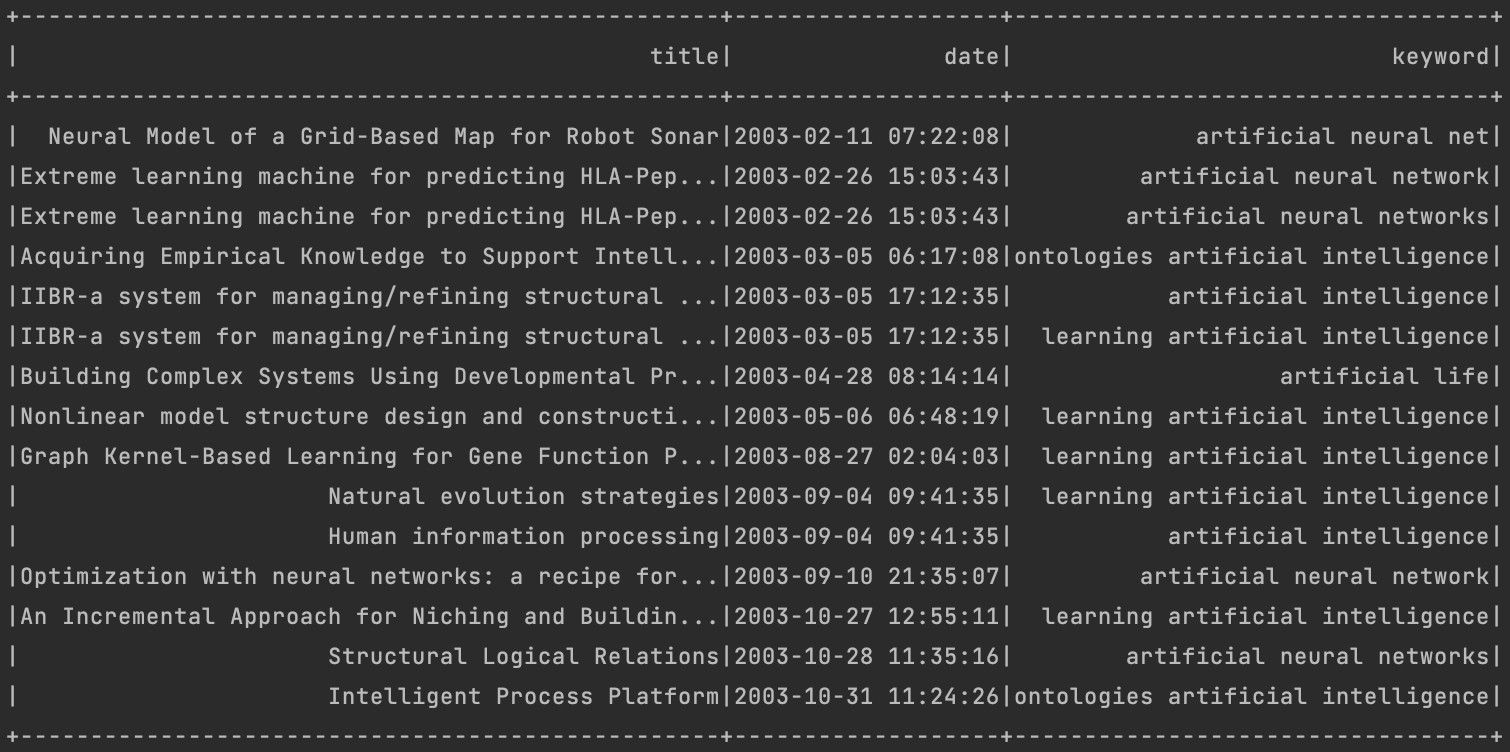
\includegraphics[width=0.9\linewidth]{ImagesSpark/query2spark}
            \label{fig:query2spark}%
        \end{center}
    \end{figure}
    \item \textbf{Retrieve papers published in conferences that have topics about multiagent systems} \\
    This query retrieves the papers with \verb|multiagent system| within its keywords, so we are interested only in a subset of our database.
    In extracting them, we select at first some of the columns of the dataframe associated with papers, and in particular, we call the explode function over the \verb|keywords| column to duplicate the rows and associate to them an element of the exploded column.
    Then, we extract a subset of all the generated rows by selecting only those that have as keyword \verb|multiagent system|.
    We extract only the columns \verb|title|, \verb|publication_type|, \verb|paper_id|, \verb|publication_id|, and \verb|date|, and we save the result in a variable called \verb|nested_query|.

    Thus, we perform another query over the created dataframe by first calling a join operation to join it with the one associated with the conferences, matching the variable \verb|publication_id|, and then we select only those papers of interest.
    We reorder the rows by date in a descending way, and then we extract only the title of the paper and the venue of the conference.
    Finally, we show the dataframe obtained.
    \begin{lstlisting}[label={lst:lstlisting4_1_8}]
nested_query = df_papers \
.select('title',
'publication_type',
'paper_id',
'publication_id',
'date',
explode('keywords').alias('keyword')) \
.filter(col('keyword').isin('multiagent system')) \
.drop('keyword')
df_conferences \
.join(nested_query, 'publication_id') \
.filter(col('publication_type') == 'Conference') \
.orderBy('date', ascending=False) \
.select(col('title').alias('paper title'),
col('venue').alias('conference venue')) \
.show(5, truncate=50)
    \end{lstlisting}
    \begin{figure}[H]
        \begin{center}
            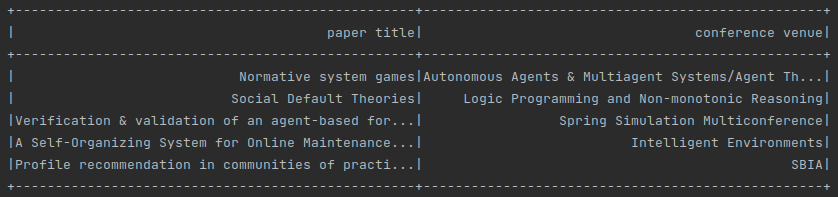
\includegraphics[width=0.9\linewidth]{ImagesSpark/query3spark}
            \label{fig:query3spark}%
        \end{center}
    \end{figure}
    \item \textbf{Retrieve the most prolific organizations regarding the conferences} \\
    This query tries to retrieve the organizations that published more than \verb|10| conferences, so the most prolific ones in these kinds of publications.
    We first execute a join between the DataFrame that contains the papers and the one that contains the affiliations, because to obtain the result we need information from them both.
    We need to filter on the \verb|publication_type| that is present in \verb|df_papers| in order to consider only the conferences and, then, we group by \verb|organization|, present in the \verb|df_aff|, and with \verb|collect_set()| we collect for each organization the list of the related papers, avoiding duplicates.
    Finally, we filter the result, retrieving only those organizations whose associated list has more than \verb|10 paper_id|.
    In showing the most prolific organizations we truncate the columns' text using \verb|truncate = 50|, to have a compact and clear visualization.
    \begin{lstlisting}[label={lst:query4spark}]
from pyspark.sql.functions import collect_set, size

df_aff \
.join(df_papers, df_papers.paper_id == df_aff.paper_id, 'inner') \
.drop(df_papers.paper_id) \
.select('paper_id',
'organization',
'publication_type') \
.filter((col('organization').isNotNull()) &
(col('organization') != "") &
(col('publication_type') == "Conference")) \
.groupBy('organization') \
.agg(collect_set('paper_id').alias('papers')) \
.filter(size(col('papers')) > 10) \
.show(truncate=50)
    \end{lstlisting}
    \begin{figure}[H]
        \begin{center}
            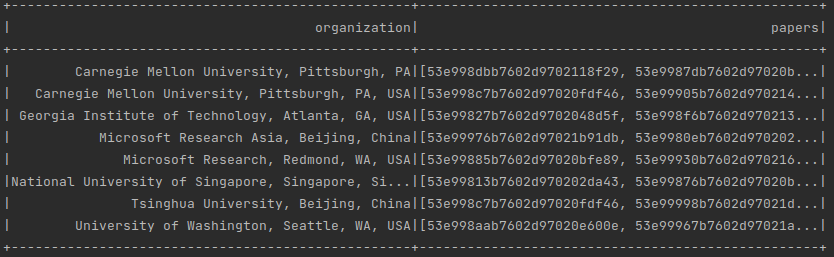
\includegraphics[width=0.9\linewidth]{ImagesSpark/query4spark}
            \label{fig:query4spark}%
        \end{center}
    \end{figure}
    \item \textbf{Retrieve some statistics about papers } \\
    In this query, we retrieve some statistics about papers published from the year 2015 on.
    We group the articles by publication year using the \verb|year()| function to extract the year from the date.
    Then some aggregate functions are performed to obtain insights like the total number of papers published using \verb|count()|, the total number of pages written, the minimum and the maximum number of pages in an article using \verb|sum()|, \verb|min()|, \verb|max()| and lastly the mean of pages written per article and the variance using \verb|avg()| and \verb|variance()|.
    To round the fractional numbers we use \verb|format_number()|.
    Years are shown in decreasing order.
    In this query we use the DataFrame obtained by running the command 5.
    \begin{lstlisting}[label={lst:query5spark}]
from pyspark.sql.functions import sum, min, max, avg, format_number, variance

df_papers_total_pages \
.filter(year(col('date')) >= 2015) \
.groupBy(year(col('date')).alias('year')) \
.agg(count('paper_id').alias('total_papers'),
sum('total_pages').alias('total_pages'),
min('total_pages').alias('min_pages'),
max('total_pages').alias('max_pages'),
format_number(avg('total_pages'), 2).alias('avg_pages'),
format_number(variance('total_pages'), 2).alias('var_pages')) \
.sort(col('year').desc()) \
.show()
    \end{lstlisting}
    \begin{figure}[H]
        \begin{center}
            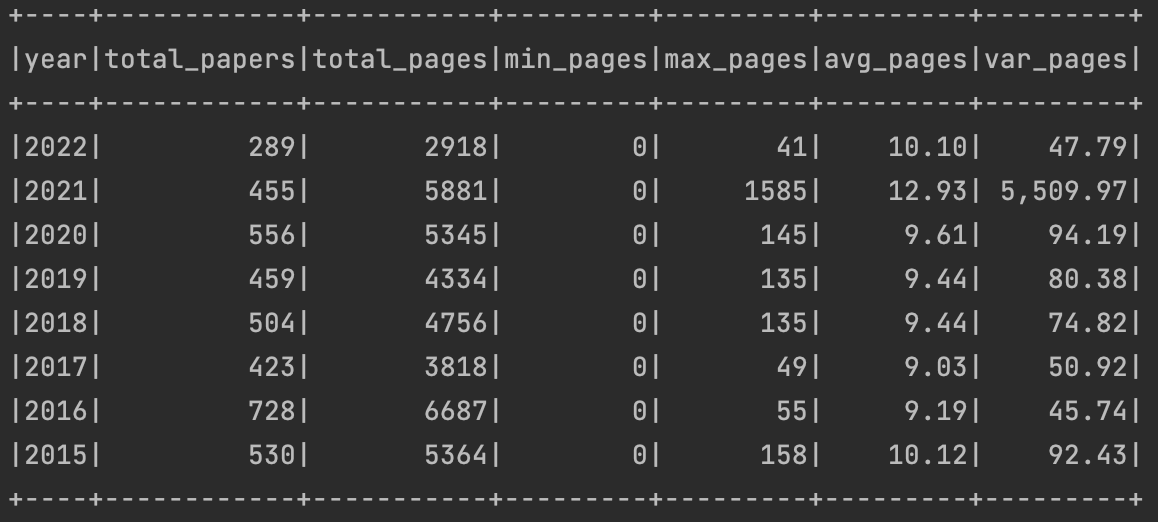
\includegraphics[width=0.9\linewidth]{ImagesSpark/query5spark}
            \label{fig:query5spark}%
        \end{center}
    \end{figure}
    \item \textbf{Papers that are referenced the most and have at least 30 references} \\
    With this query, we want to know which papers present in our DB are referenced the most absolute ly.
    We achieve this goal by first unwrapping the references for each paper using the \verb|explode| function.
    Then, we proceed grouping by the reference we previously \textit{exploded} and use the \verb|count| aggregation function to actually count the papers who have that particular reference, saving this value in the column \verb|references_count|.
    Lastly, we do a filtering on \verb|references_count| to extract only the papers with at least 30 references, and a join to get some significant data about the papers we extracted with the previous operations.
    \begin{lstlisting}[label={lst:query6spark}]
df_papers \
.select('paper_id',
'title',
explode(col('references')).alias('reference')) \
.groupBy('reference') \
.agg(count('paper_id').alias('references_count')) \
.filter(col('references_count') > 30) \
.join(df_papers, col('reference') == df_papers.paper_id) \
.sort(col('references_count').desc()) \
.select(['title', 'references_count']) \
.show(truncate=50)
    \end{lstlisting}
    \begin{figure}[H]
        \begin{center}
            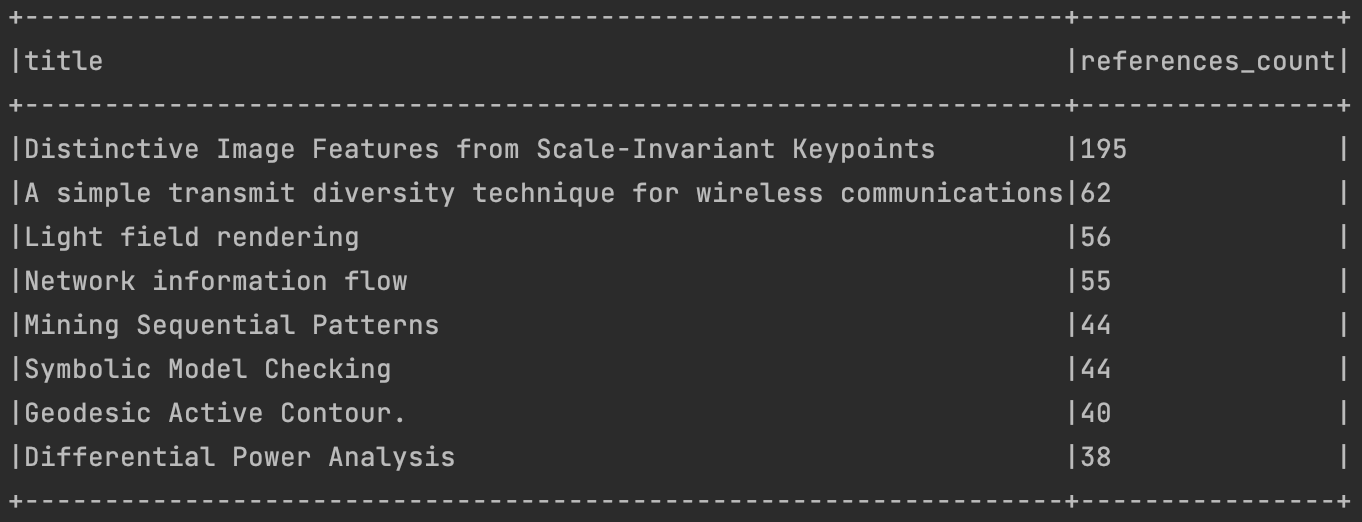
\includegraphics[width=0.9\linewidth]{ImagesSpark/query6spark}
            \label{fig:query6spark}%
        \end{center}
    \end{figure}
    \item \textbf{Couples of the field of study and keywords which appear more frequently within the papers} \\
    The query returns the association between fields of study and keywords which are more present inside the database and how many times they appear together.
    Initial filtering is done in order to eliminate the papers which don't contain any keyword or field of study.
    The two clauses for doing the filtering can be modified by increasing the required number of keywords or the required number of fields of study.
    This kind of change can be interesting in order to understand which fields of study and keywords become more relevant when the subset of the considered paper is different.
    The results are ordered by the number of occurrences of the couples \verb|field of study| - \verb|keyword| by decreasing order.
    We filter out the couples of fields of study and keywords with less than 100 occurrences in order to get rid of some misleading information due to not coupled elements.
    The threshold can be adjusted.
    \begin{lstlisting}[label={lst:query7spark}]
from pyspark.sql.functions import year, col, size

df = df_papers \
.filter(
(col('doi').isNotNull()) &
(year(col('date')) >= 2000) &
(size(col('fos')) > 0) &
(size(col('keywords')) > 0)) \
.select('fos', explode('keywords').alias('keyword')) \
.select('keyword', explode('fos').alias('fos')) \
.groupby('fos', 'keyword') \
.count() \
.withColumnRenamed('count', 'couple count') \
.filter(col('couple count') > 100) \
.sort(col('couple count').desc()) \
.limit(15) \
.show(truncate=False)
    \end{lstlisting}
    \begin{figure}[H]
        \begin{center}
            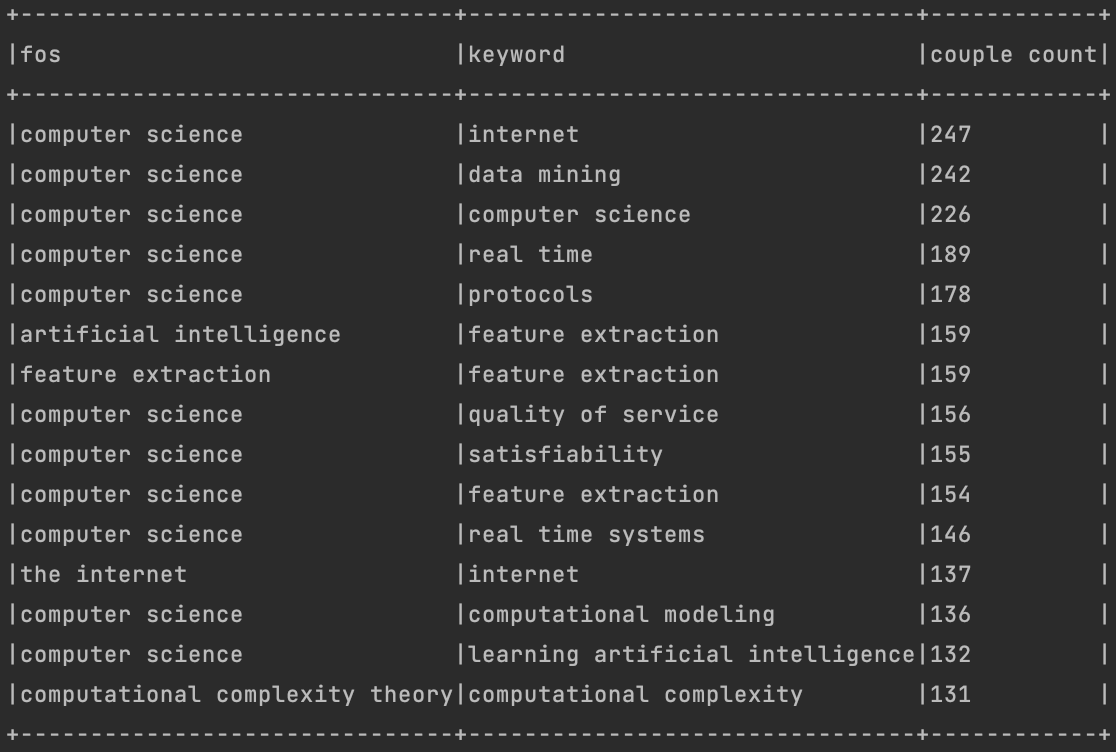
\includegraphics[width=0.9\linewidth]{ImagesSpark/query7spark}
            \label{fig:query7spark}%
        \end{center}
    \end{figure}
    \item \textbf{Retrieve the organizations associated with an author name for each field of study} \\
    For each field of study associated with papers written by any author named \verb|Hao Wang|, this query retrieves all the organizations that have contributed to that field of study through the searched authors.

    For the complexity of the problem, we split the query into two nested queries.
    At first, we query the data frame associated with authors by filtering it to extract the author \verb|Hao Wang|.
    Then we select only the \verb|author_id| column, and we collect the values in a list called \verb|sub_nested_query| through the functions \verb|flatMap| and \verb|collect|.

    Next, we are interested in filtering also the data frame associated with affiliation by extracting rows that have \verb|author_id| present inside the \verb|sub_nested_query| list.
    We also filter the same data frame by extracting only the rows with a not-null value of the organization column, and then we assign the result to the \verb|nested_query| variable.

    Finally, we join over the column \verb|paper_id| the last result with the data frame associated with papers.
    From the joined data frame, we explode the column \verb|fos|, and we associate to each of those elements called \verb|field_of_study| the value of the columns \verb|paper_id| and \verb|organization|.
    We group the rows by the \verb|field_of_study| values, and then we aggregate through the function \verb|agg| the organizations that are collected in a set by the last operation.
    We are performing these operations because we are interested in all the organizations in which the author has worked in his carrier.
    In the end, we rearrange the rows by ordering the column \verb|field_of_study| alphabetically.
    \begin{lstlisting}[label={lst:query8spark}]
author_name = 'Hao Wang'

sub_nested_query = df_aut \
.filter(col('name') == author_name) \
.select('author_id') \
.rdd.flatMap(lambda x: x) \
.collect()

nested_query = df_aff \
.filter(col('author_id').isin(sub_nested_query)) \
.filter(col('organization') != 'null')

df_papers \
.join(nested_query, 'paper_id') \
.select('paper_id',
'organization',
explode('fos').alias('field_of_study')) \
.groupBy('field_of_study') \
.agg(collect_set('organization').alias('organization')) \
.orderBy('field_of_study') \
.show(14, truncate=80)
    \end{lstlisting}
    \begin{figure}[H]
        \begin{center}
            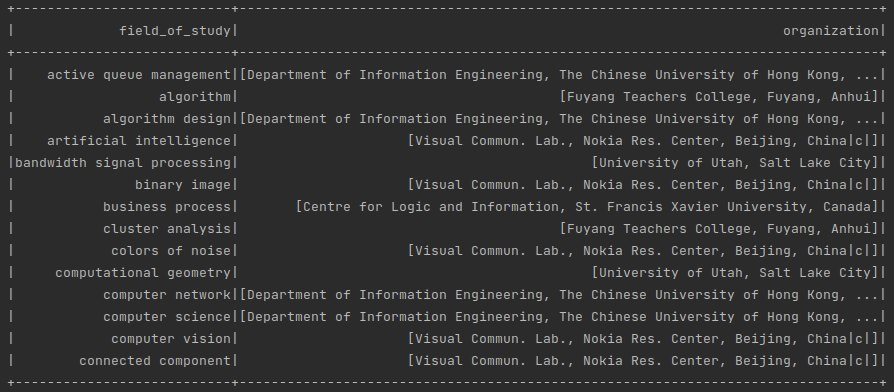
\includegraphics[width=0.9\linewidth]{ImagesSpark/query8spark}
            \label{fig:query8spark}%
        \end{center}
    \end{figure}
    \item \textbf{Retrieve the most prolific publishers} \\
    In this query, we join the \verb|df_books| and the \verb|df_journals| on the \verb|publisher| column.
    Due to this join and to the fact that the two DataFrames have both the column \verb|venue| we have to rename this column in at least one of the tables, to have distinguishable data.
    We decided to rename both columns to have more clear data in the new DataFrame, created by the join operation.
    In this case, combining the related tuples from books and journals, we are interested only in journals' publications that arrived at least at volume \verb|10|, while we consider all the books without filtering them.
    After the execution of the join, we drop the duplicates and group them by \verb|publisher|.
    Then, we create two sets related to the publisher, one for the books and one for the journals, and we concatenate them to obtain for each publisher a single list with all its publications.
    We define sets and not lists because they don't allow to have duplicates of values.
    Now, we can retrieve the most prolific publishers, just by filtering on the size of the list of publications associated with the publishers.
    In our dataset, there are not a lot of publishers that have more than \verb|500| publications, so these are the most prolific ones, but the filtering can be modified at any time, depending on the data, to obtain meaningful results.
    \begin{lstlisting}[label={lst:query9spark}]
from pyspark.sql.functions import collect_set, concat, size

df_journals \
.withColumnRenamed('venue', 'venueJournals') \
.filter((col('volume')) > 10) \
.join(df_books, df_books.publisher == df_journals.publisher, 'inner') \
.drop(df_journals.publisher) \
.withColumnRenamed('venue', 'venueBooks') \
.select('venueBooks',
'venueJournals',
'publisher') \
.dropDuplicates(['venueBooks',
'venueJournals',
'publisher']) \
.groupBy('publisher') \
.agg(collect_set('venueBooks').alias('books'),
collect_set('venueJournals').alias('journals')) \
.withColumn('total_publications_per_publisher', concat('books', 'journals')) \
.filter(size('total_publications_per_publisher') > '500') \
.select('publisher',
'total_publications_per_publisher') \
.show(truncate=50)
    \end{lstlisting}
    \begin{figure}[H]
        \begin{center}
            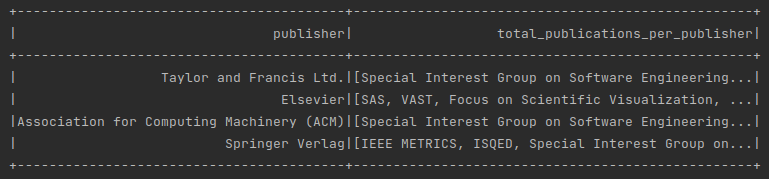
\includegraphics[width=0.9\linewidth]{ImagesSpark/query9spark}
            \label{fig:query9spark}%
        \end{center}
    \end{figure}
    \item \textbf{Prolific authors with different organizations} \\
    The query retrieves authors who worked for at least three different organizations and have published at least three papers with at least five fields of study and five references each.
    To obtain this it is necessary to join the paper table with the affiliation DataFrame on \verb|paper_id| and then join it with the author DataFrame on \verb|author_id|.
    We group on \verb|author_id| to get all the aggregate information for each author.
    To count the different organizations an author has worked for we use \verb|approx_count_distinct()|, which gives a faster response counting approximately the different values, if interested in the exact value it is possible to use \verb|countDistinct()|.
    In the \verb|HAVING| part, for consistency, we check that only one name is associated with the grouped \verb|author_id| and in the \verb|SELECT| part we explode that field to obtain a single string instead of an array.
    The result is decreasingly ordered by the number of papers and then the number of organizations.
    \begin{lstlisting}[label={lst:query10spark}]
from pyspark.sql.functions import approx_count_distinct

df_papers \
.filter((size(col('fos')) >= 5) &
(size(col('references')) >= 5)) \
.join(df_aff, df_papers.paper_id == df_aff.paper_id, 'inner') \
.drop(df_aff.paper_id) \
.join(df_aut, df_aff.author_id == df_aut.author_id, 'inner') \
.drop(df_aff.author_id) \
.groupBy('author_id') \
.agg(count('paper_id').alias('papers_count'),
approx_count_distinct('organization').alias('organizations_count'),
collect_set('name').alias('name')) \
.filter((size('name') == 1) &
(col('papers_count') >= 3) &
(col('organizations_count') >= 3)) \
.orderBy(col('papers_count').desc(),
col('organizations_count').desc()) \
.select(explode('name').alias('name'),
'papers_count',
'organizations_count') \
.show(5)
    \end{lstlisting}
    \begin{figure}[H]
        \begin{center}
            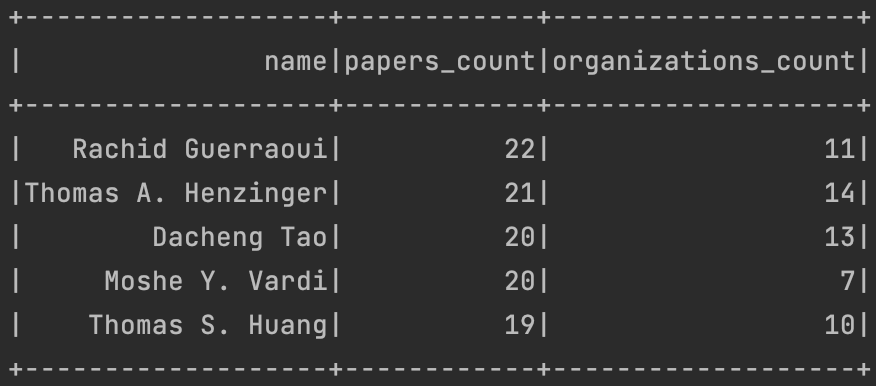
\includegraphics[width=0.9\linewidth]{ImagesSpark/query10spark}
            \label{fig:query10spark}%
        \end{center}
    \end{figure}
\end{enumerate}
